% !TEX TS-program = latexmk
\documentclass[11pt,a4paper]{report}

\usepackage[a4paper,margin=1in]{geometry}
\usepackage{microtype}
\usepackage{amsmath}
\usepackage{amssymb}
\usepackage{mathtools}
\usepackage{graphicx}
\usepackage{caption}
\usepackage{subcaption}
\usepackage{tikz}
\usepackage{booktabs}
\usepackage{tabularx}
\usepackage{longtable}
\usepackage{siunitx}
\usepackage[colorlinks=true,linkcolor=blue!50!black,citecolor=blue!50!black,urlcolor=blue!50!black]{hyperref}

\newif\ifReportBiblatexLoaded
\IfFileExists{biblatex.sty}{%
  \ReportBiblatexLoadedtrue
  \usepackage[backend=biber,style=ieee,sorting=none]{biblatex}
  \addbibresource{bib/references.bib}
}{%
  \ReportBiblatexLoadedfalse
}

\graphicspath{{figures/}}

\captionsetup{font=small,labelfont=bf}
\setlength{\parindent}{0pt}
\setlength{\parskip}{0.55em}
\numberwithin{equation}{chapter}

\sisetup{
  detect-all,
  per-mode=symbol,
  round-mode=places,
  round-precision=3
}

\providecommand{\ReportTitle}{Ball and Beam Experiment Report}
\providecommand{\ReportSubtitle}{Self-contained multi-file LaTeX engineering report}
\providecommand{\ReportAuthor}{Author Name}
\providecommand{\ReportInstitution}{Institution / Lab}
\providecommand{\ReportDate}{\today}

\providecommand{\TelemetryRowCount}{0}
\providecommand{\TelemetryClosedLoopRowCount}{0}
\providecommand{\TelemetryDurationSeconds}{0.0}
\providecommand{\TelemetryInvalidRowCount}{0}
\providecommand{\TelemetryRecoveryRowCount}{0}
\providecommand{\TelemetryFarValidCount}{0}
\providecommand{\TelemetryFarTotalCount}{0}
\providecommand{\TelemetryCenterValidCount}{0}
\providecommand{\TelemetryCenterTotalCount}{0}
\providecommand{\TelemetryNearValidCount}{0}
\providecommand{\TelemetryNearTotalCount}{0}
\providecommand{\CalibrationPointCount}{0}
\providecommand{\CalibrationMeanHysteresisDeg}{0.0}
\providecommand{\CalibrationMaxHysteresisDeg}{0.0}
\providecommand{\CalibrationRmsHysteresisDeg}{0.0}
\providecommand{\TelemetryMaxAbsErrorCm}{0.0}
\providecommand{\TelemetryMaxBeamAngleDeg}{0.0}
\providecommand{\TelemetryMaxCommandDeg}{0.0}

\newcommand{\MissingAssetPlaceholder}[2][0.82\linewidth]{%
  \begin{center}
    \setlength{\fboxsep}{10pt}%
    \fbox{%
      \begin{minipage}{#1}
        \centering
        \textbf{Placeholder asset}\\[0.5em]
        #2
      \end{minipage}%
    }%
  \end{center}
}

\newcommand{\ReportFigure}[4][]{%
  \begin{figure}[tbp]
    \centering
    \IfFileExists{#2}{%
      \includegraphics[#1]{#2}%
    }{%
      \MissingAssetPlaceholder{Missing figure file \texttt{\detokenize{#2}}.}%
    }%
    \caption{#3}
    \label{#4}
  \end{figure}
}

\newcommand{\ReportTableFromFile}[3]{%
  \begin{table}[tbp]
    \centering
    \caption{#1}
    \label{#3}
    \IfFileExists{#2}{%
      \input{#2}%
    }{%
      \MissingAssetPlaceholder[0.70\linewidth]{Missing table file \texttt{\detokenize{#2}}.}%
    }%
  \end{table}
}

\newcommand{\ReportPrintBibliography}{%
  \clearpage
  \chapter*{References}
  \addcontentsline{toc}{chapter}{References}
  \ifReportBiblatexLoaded
    \IfFileExists{build/main.bbl}{%
    \nocite{*}%
    \printbibliography[heading=none]%
    }{%
      \begin{thebibliography}{99}
        \bibitem{franklin2015feedback}
G.~F. Franklin, J.~D. Powell, and A.~Emami-Naeini, \emph{Feedback Control of Dynamic Systems}, 7th~ed. Pearson, 2015.

\bibitem{astrom2010feedback}
K.~J. {\AA}str{\"o}m and R.~M. Murray, \emph{Feedback Systems: An Introduction for Scientists and Engineers}. Princeton University Press, 2010.

\bibitem{sharpgp2y0a41}
Sharp Corporation, ``GP2Y0A41SK0F distance measuring sensor unit datasheet,'' 2019.

\bibitem{amsas5600}
ams OSRAM, ``AS5600 magnetic rotary position sensor datasheet,'' 2021.

\bibitem{tmc2209}
TRINAMIC Motion Control GmbH, ``TMC2209 datasheet,'' 2020.

      \end{thebibliography}
    }%
  \else
    \begin{thebibliography}{99}
      \bibitem{franklin2015feedback}
G.~F. Franklin, J.~D. Powell, and A.~Emami-Naeini, \emph{Feedback Control of Dynamic Systems}, 7th~ed. Pearson, 2015.

\bibitem{astrom2010feedback}
K.~J. {\AA}str{\"o}m and R.~M. Murray, \emph{Feedback Systems: An Introduction for Scientists and Engineers}. Princeton University Press, 2010.

\bibitem{sharpgp2y0a41}
Sharp Corporation, ``GP2Y0A41SK0F distance measuring sensor unit datasheet,'' 2019.

\bibitem{amsas5600}
ams OSRAM, ``AS5600 magnetic rotary position sensor datasheet,'' 2021.

\bibitem{tmc2209}
TRINAMIC Motion Control GmbH, ``TMC2209 datasheet,'' 2020.

    \end{thebibliography}
  \fi
}

\IfFileExists{metadata.tex}{\renewcommand{\ReportTitle}{Ball and Beam Experiment Report}
\renewcommand{\ReportSubtitle}{Modeling, calibration, control implementation, and April 11 telemetry results}
\renewcommand{\ReportAuthor}{Author Name}
\renewcommand{\ReportInstitution}{Institution / Lab}
\renewcommand{\ReportDate}{\today}
}{}
\IfFileExists{tables/generated_macros.tex}{\renewcommand{\TelemetryRowCount}{364}
\renewcommand{\TelemetryClosedLoopRowCount}{350}
\renewcommand{\TelemetryDurationSeconds}{72.601}
\renewcommand{\TelemetryInvalidRowCount}{43}
\renewcommand{\TelemetryRecoveryRowCount}{9}
\renewcommand{\TelemetryFarValidCount}{59}
\renewcommand{\TelemetryFarTotalCount}{100}
\renewcommand{\TelemetryCenterValidCount}{98}
\renewcommand{\TelemetryCenterTotalCount}{100}
\renewcommand{\TelemetryNearValidCount}{119}
\renewcommand{\TelemetryNearTotalCount}{119}
\renewcommand{\CalibrationPointCount}{112}
\renewcommand{\CalibrationMeanHysteresisDeg}{0.418}
\renewcommand{\CalibrationMaxHysteresisDeg}{0.600}
\renewcommand{\CalibrationRmsHysteresisDeg}{0.422}
\renewcommand{\TelemetryMaxAbsErrorCm}{3.712}
\renewcommand{\TelemetryMaxBeamAngleDeg}{1.543}
\renewcommand{\TelemetryMaxCommandDeg}{1.344}
}{}

\begin{document}

\pagenumbering{gobble}
\begin{titlepage}
    \centering
    \vspace*{2.5cm}
    {\Huge\bfseries \ReportTitle\par}
    \vspace{0.6cm}
    {\Large \ReportSubtitle\par}
    \vspace{1.8cm}
    {\large \ReportAuthor\par}
    \vspace{0.4cm}
    {\large \ReportInstitution\par}
    \vfill
    {\large \ReportDate\par}
    \vspace*{1cm}
\end{titlepage}

\pagenumbering{roman}
\setcounter{page}{1}
\tableofcontents
\clearpage
\listoffigures
\clearpage
\listoftables
\clearpage

\pagenumbering{arabic}

% !TEX root = ../main.tex
\chapter{Introduction}

This document provides a standalone engineering report system for the ball and beam
experiment contained in this repository. The report combines the canonical modeling
record in \path{modeling.md}, calibration evidence from the April 7, 2026 beam-angle
campaign, and the staircase telemetry run stored in
\path{telemetry_logs/20260411_142117/telemetry.csv}.

The report structure is intentionally self-contained. All LaTeX sources, bibliography
files, generated figures, generated tables, and build outputs live inside
\path{report/}. The analysis pipeline reads the raw CSV logs directly and exports
report-ready plots and tabular summaries without depending on any other repository.

\section{Purpose}

The main goals are:

\begin{itemize}
  \item capture the first-principles ball and beam model used for the project,
  \item document the implemented sensing, calibration, and cascaded controller in
  the firmware,
  \item analyze the available calibration and staircase telemetry logs directly from
  raw CSV data, and
  \item provide a maintainable report build flow that works from the terminal and in
  VS Code with LaTeX Workshop.
\end{itemize}

\section{Data Sources}

The report uses the following repository-local sources as its primary experiment record:

\begin{itemize}
  \item \path{modeling.md} for the mathematical derivation, sign conventions, and
  implementation record,
  \item \path{src/main.cpp} for the shipped controller constants and mode logic,
  \item \path{telemetry_logs/20260411_142117/telemetry.csv} for the closed-loop
  staircase experiment, and
  \item \path{calibration_logs/combined_20260407_forward_reverse/combined_cleaned_calibration.csv}
  for beam-angle calibration hysteresis characterization.
\end{itemize}

\section{Report Roadmap}

Chapter~2 summarizes the physical apparatus, coordinates, and measured parameters.
Chapter~3 reproduces the nonlinear derivation from the canonical model record.
Chapter~4 specializes the model around the horizontal operating point for control
design. Chapter~5 documents the firmware implementation actually used in the hardware
run. Chapter~6 analyzes the beam-angle calibration data. Chapter~7 discusses the April
11 telemetry run using plots and performance metrics generated directly from the raw
CSV logs. Chapter~8 closes with key findings and immediate next steps.

% !TEX root = ../main.tex
\chapter{System Description}

\section{Physical Arrangement}

The apparatus is a single-axis ball and beam system. A ping-pong ball rolls along a
V-groove runner mounted on an aluminum beam. The beam pivots near the Sharp IR sensor
end and is actuated at the far end by a NEMA 17 stepper motor through a linkage. The
IR sensor measures ball distance from its sensing face, while an AS5600 magnetic sensor
measures beam angle on the actuator side.

\begin{figure}[tbp]
  \centering
  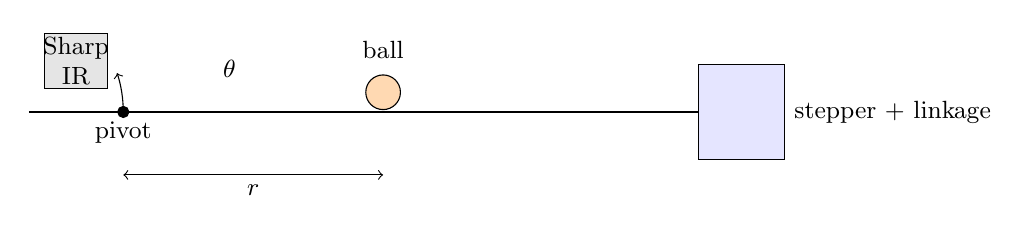
\begin{tikzpicture}[scale=1.0, every node/.style={font=\small}]
    \draw[thick] (0,0) -- (9,0);
    \filldraw[black] (1.2,0) circle (2pt);
    \node[below] at (1.2,0) {pivot};
    \draw[fill=gray!20] (0.2,0.3) rectangle (1.0,1.0);
    \node[align=center] at (0.6,0.65) {Sharp\\IR};
    \draw[fill=orange!30] (4.5,0.25) circle (0.22);
    \node[above] at (4.5,0.55) {ball};
    \draw[fill=blue!10] (8.5,-0.6) rectangle (9.6,0.6);
    \node[right] at (9.6,0) {stepper + linkage};
    \draw[<->] (1.2,-0.8) -- (4.5,-0.8);
    \node[below] at (2.85,-0.8) {$r$};
    \draw[->] (1.2,0.0) arc[start angle=0,end angle=18,radius=1.6];
    \node at (2.55,0.55) {$\theta$};
  \end{tikzpicture}
  \caption{Simplified ball and beam geometry used throughout the report. Positive
  ball position is measured away from the pivot; positive analytical beam angle raises
  the motor side.}
  \label{fig:system_geometry}
\end{figure}

\section{Coordinates and Sign Convention}

The generalized coordinates are the ball position $r$ measured from the pivot and the
beam angle $\theta$ measured from the horizontal. The analytical sign convention from
\path{modeling.md} is:

\begin{itemize}
  \item $r > 0$ means the ball is farther from the pivot and closer to the motor end.
  \item $\theta > 0$ means the motor side of the beam is up.
  \item Under this analytical convention, positive $\theta$ makes gravity pull the
  ball toward the pivot, so $r$ decreases.
\end{itemize}

The firmware uses a calibrated runtime angle \verb|theta_rel_deg| whose sign is the
opposite of the analytical small-angle model. That distinction is kept explicit in the
control chapters so the mechanics remain clean while the implementation record stays
faithful to the hardware.

\section{Measured Hardware Parameters}

Table~\ref{tab:raw_measurements} summarizes the measured geometric and inertial values
used in the model.

\begin{table}[tbp]
  \centering
  \small
  \caption{Measured hardware parameters taken from the canonical modeling record.}
  \label{tab:raw_measurements}
  \begin{tabularx}{\linewidth}{@{}l c X@{}}
    \toprule
    Quantity & Value & Notes \\
    \midrule
    Ball mass & \SI{2.8}{g} & Standard \SI{40}{mm} ping-pong ball \\
    Ball diameter & \SI{40.0}{mm} & Hollow thin-shell approximation \\
    Bare beam mass & \SI{33.2}{g} & Aluminum extrusion over \SI{263}{mm} span \\
    Sensor plus wires mass & \SI{5.3}{g} & Pivot-mounted Sharp assembly \\
    Total beam assembly mass & \SI{38.5}{g} & Beam, sensor, and wiring lumped together \\
    Beam length & \SI{263}{mm} & Clevis to clevis \\
    Sensor face from pivot & \SI{40.3}{mm} & Reference for the distance measurement \\
    Nearest usable ball distance from sensor & \SI{44.0}{mm} & Tape stop prevents foldback region \\
    Farthest usable ball distance from sensor & \SI{126.6}{mm} & Far stop in the tested runner window \\
    Stepper resolution & \num{3200} microsteps/rev & \num{200} full steps with 1/16 microstepping \\
    Rolling viscous damping & \SI{0.0125}{N.s/m} & Pre-identification estimate \\
    Pivot viscous damping & \SI{0.006}{N.m.s} & Pre-identification estimate \\
    \bottomrule
  \end{tabularx}
\end{table}

The corresponding evaluated SI parameters used later are:

\begin{itemize}
  \item ball radius $R = \SI{0.020}{m}$,
  \item ball inertia $I = \tfrac{2}{3} m R^2 = \SI{7.467e-7}{kg.m^2}$,
  \item beam assembly mass $M_b = \SI{0.0385}{kg}$,
  \item beam center of mass $L_{\text{com}} = \SI{0.11805}{m}$,
  \item beam inertia about the pivot $J = \SI{7.715e-4}{kg.m^2}$, and
  \item nominal center operating point $r_0 = \SI{0.1256}{m}$.
\end{itemize}

\section{Controller-Relevant Coordinate Translation}

The firmware record in \path{modeling.md} and \path{src/main.cpp} defines:

\begin{align}
  \theta_{\text{cal,deg}} &= 0.07666806 \cdot \theta_{\text{AS5600,deg}} - 23.28443907 \\
  \theta_{\text{rel,deg}} &= \theta_{\text{cal,deg}} - \theta_{\text{balance,deg}} \\
  x_{\text{cm}} &= d_{\text{filt,cm}} - d_{\text{setpoint,cm}}
\end{align}

with the empirically verified meanings:

\begin{itemize}
  \item $x_{\text{cm}} > 0$ means the ball is toward the motor end,
  \item manual command \verb|A+| rolls the ball toward the motor end, and
  \item near the operating point, $\theta_{\text{rel,deg}} \approx -\theta_{\text{phys,deg}}$.
\end{itemize}

This split between analytical and firmware coordinates is central to interpreting both
the model and the telemetry correctly.

% !TEX root = ../main.tex
\chapter{Nonlinear Modeling and Derivation}

\section{Kinematics}

With the pivot taken as the origin of an inertial frame, the ball center coordinates are

\begin{align}
  x_I &= r \cos \theta \\
  y_I &= r \sin \theta
\end{align}

where $r$ is the distance of the ball along the beam and $\theta$ is the beam angle from
horizontal.

Differentiating gives the inertial velocity components:

\begin{align}
  \dot{x}_I &= \dot{r}\cos\theta - r\dot{\theta}\sin\theta \\
  \dot{y}_I &= \dot{r}\sin\theta + r\dot{\theta}\cos\theta
\end{align}

The squared speed simplifies to the standard polar-coordinate result:

\begin{align}
  v^2
  &= \dot{x}_I^2 + \dot{y}_I^2 \\
  &= \left(\dot{r}\cos\theta - r\dot{\theta}\sin\theta\right)^2
   + \left(\dot{r}\sin\theta + r\dot{\theta}\cos\theta\right)^2 \\
  &= \dot{r}^2 + r^2 \dot{\theta}^2
\end{align}

The ball is modeled as rolling without slip along the beam, so its spin rate is

\begin{equation}
  \omega_{\text{ball}} = \frac{\dot{r}}{R}
\end{equation}

This removes the ball spin as an independent degree of freedom.

\section{Energy Terms}

\subsection{Ball Translational and Rotational Kinetic Energy}

The translational kinetic energy is

\begin{equation}
  T_{\text{trans}} = \frac{1}{2} m \left(\dot{r}^2 + r^2\dot{\theta}^2\right)
\end{equation}

Using the thin-shell inertia $I = \tfrac{2}{3}mR^2$ and the rolling constraint, the
rotational kinetic energy becomes

\begin{align}
  T_{\text{rot}}
  &= \frac{1}{2} I \omega_{\text{ball}}^2 \\
  &= \frac{1}{2}\left(\frac{2}{3}mR^2\right)\left(\frac{\dot{r}}{R}\right)^2 \\
  &= \frac{1}{3} m \dot{r}^2
\end{align}

\subsection{Beam Kinetic Energy}

The beam assembly rotates as a rigid body about the pivot:

\begin{equation}
  T_{\text{beam}} = \frac{1}{2} J \dot{\theta}^2
\end{equation}

\subsection{Total Kinetic Energy}

Summing all contributions gives

\begin{align}
  T
  &= T_{\text{trans}} + T_{\text{rot}} + T_{\text{beam}} \\
  &= \frac{5}{6}m\dot{r}^2 + \frac{1}{2}\left(mr^2 + J\right)\dot{\theta}^2
\end{align}

The $\tfrac{5}{6}$ factor on $\dot{r}^2$ is the characteristic effective-mass term of
the ball and beam plant.

\subsection{Potential Energy}

Taking the pivot height as the reference, the ball and beam potential energies are

\begin{align}
  V_{\text{ball}} &= mgr\sin\theta \\
  V_{\text{beam}} &= M_b g L_{\text{com}} \sin\theta
\end{align}

so the total potential energy is

\begin{equation}
  V = (mr + M_bL_{\text{com}}) g \sin\theta
\end{equation}

\subsection{Lagrangian}

The Lagrangian is therefore

\begin{equation}
  \mathcal{L}
  = \frac{5}{6}m\dot{r}^2
  + \frac{1}{2}\left(mr^2 + J\right)\dot{\theta}^2
  - (mr + M_bL_{\text{com}}) g \sin\theta
\end{equation}

\section{Euler--Lagrange Equations}

The generalized forces include viscous rolling damping and actuator torque:

\begin{align}
  Q_r &= -b_x \dot{r} \\
  Q_{\theta} &= \tau - b_{\theta}\dot{\theta}
\end{align}

\subsection{Ball Equation}

For the $r$ coordinate,

\begin{align}
  \frac{\partial \mathcal{L}}{\partial \dot{r}} &= \frac{5}{3}m\dot{r} \\
  \frac{d}{dt}\left(\frac{\partial \mathcal{L}}{\partial \dot{r}}\right) &= \frac{5}{3}m\ddot{r} \\
  \frac{\partial \mathcal{L}}{\partial r} &= mr\dot{\theta}^2 - mg\sin\theta
\end{align}

Applying the Euler--Lagrange equation yields

\begin{equation}
  \frac{5}{3}m\ddot{r} + b_x\dot{r} - mr\dot{\theta}^2 + mg\sin\theta = 0
  \label{eq:eom_r}
\end{equation}

The terms represent the effective rolling inertia, viscous damping, centrifugal
coupling from beam rotation, and gravitational acceleration along the beam.

\subsection{Beam Equation}

For the $\theta$ coordinate,

\begin{align}
  \frac{\partial \mathcal{L}}{\partial \dot{\theta}} &= (mr^2 + J)\dot{\theta} \\
  \frac{d}{dt}\left(\frac{\partial \mathcal{L}}{\partial \dot{\theta}}\right)
    &= (mr^2 + J)\ddot{\theta} + 2mr\dot{r}\dot{\theta} \\
  \frac{\partial \mathcal{L}}{\partial \theta}
    &= -(mr + M_bL_{\text{com}})g\cos\theta
\end{align}

Hence

\begin{equation}
  (J + mr^2)\ddot{\theta}
  + 2mr\dot{r}\dot{\theta}
  + b_{\theta}\dot{\theta}
  + (mr + M_bL_{\text{com}})g\cos\theta
  = \tau
  \label{eq:eom_theta}
\end{equation}

The beam equation captures inertia variation with ball position, Coriolis coupling,
pivot damping, gravity, and motor torque.

\section{Explicit Nonlinear State Model}

Defining the effective rolling mass

\begin{equation}
  m_e = \frac{5}{3}m = \SI{0.004667}{kg}
\end{equation}

the ball equation can be written explicitly as

\begin{equation}
  \ddot{r}
  = \frac{mr\dot{\theta}^2}{m_e}
  - \frac{mg}{m_e}\sin\theta
  - \frac{b_x}{m_e}\dot{r}
\end{equation}

and the beam equation becomes

\begin{equation}
  \ddot{\theta}
  =
  \frac{
    \tau
    - 2mr\dot{r}\dot{\theta}
    - b_{\theta}\dot{\theta}
    - (mr + M_bL_{\text{com}})g\cos\theta
  }{J + mr^2}
\end{equation}

Together, these equations form the coupled nonlinear plant with state
$[r,\dot{r},\theta,\dot{\theta}]^{\mathsf{T}}$. They are the source model used for the
linearized design discussion and for interpreting the runtime controller structure.

% !TEX root = ../main.tex
\chapter{Linearization and Numerical Specialization}

\section{Operating Point}

The control design operating point is the horizontal beam equilibrium with the ball at
rest at the center of the usable sensing window:

\begin{equation}
  r = r_0 = \SI{0.1256}{m}, \qquad
  \theta = 0, \qquad
  \dot{r} = 0, \qquad
  \dot{\theta} = 0
\end{equation}

At this operating point the actuator must balance gravity with

\begin{equation}
  \tau_0 = (mr_0 + M_bL_{\text{com}})g
\end{equation}

In the implemented cascaded controller, this equilibrium torque is handled implicitly
through the beam-angle servo and balance-zero procedure.

\section{Perturbation Variables}

Define small deviations from equilibrium by

\begin{align}
  r &= r_0 + x \\
  \theta &= \delta \\
  \dot{r} &= \dot{x} \\
  \dot{\theta} &= \dot{\delta}
\end{align}

Substituting these expressions into the nonlinear equations and neglecting second-order
products gives the linearized model.

\section{Linearized Ball Dynamics}

Starting from \eqref{eq:eom_r}:

\begin{equation}
  \frac{5}{3}m\ddot{x} + b_x\dot{x} + mg\delta = 0
\end{equation}

Dividing through by the effective rolling mass $m_e = \tfrac{5}{3}m$ gives

\begin{equation}
  \ddot{x} + \beta \dot{x} = -\alpha g \delta
  \label{eq:linear_ball}
\end{equation}

with

\begin{align}
  \alpha &= \frac{m}{m_e} = \frac{3}{5} = 0.6 \\
  \beta &= \frac{b_x}{m_e} = \frac{0.0125}{0.0046667} = \SI{2.6786}{s^{-1}}
\end{align}

Numerically, the ball-position plant becomes

\begin{equation}
  \ddot{x} + 2.6786\dot{x} = -5.886\,\delta
\end{equation}

or in transfer-function form,

\begin{equation}
  \frac{X(s)}{\Theta(s)} =
  \frac{-5.886}{s^2 + 2.6786s}
  = \frac{-5.886}{s(s + 2.6786)}
\end{equation}

\section{Linearized Beam Dynamics}

Linearizing \eqref{eq:eom_theta} gives

\begin{equation}
  (J + mr_0^2)\ddot{\delta}
  + b_{\theta}\dot{\delta}
  + (mr_0 + M_bL_{\text{com}})g\delta
  = \tau - \tau_0
  \label{eq:linear_beam}
\end{equation}

Substituting the evaluated parameters yields

\begin{align}
  J_{\text{total}}(r_0)
    &= J + mr_0^2
     = \SI{8.157e-4}{kg.m^2} \\
  (mr_0 + M_bL_{\text{com}})g
    &= \SI{0.04804}{N.m/rad}
\end{align}

Ignoring damping for an estimate, the beam mode has natural frequency

\begin{equation}
  \omega_{\text{beam}}
  = \sqrt{\frac{0.04804}{8.157\times 10^{-4}}}
  = \SI{7.67}{rad/s}
  \approx \SI{1.22}{Hz}
\end{equation}

\section{Specialized Parameters}

Table~\ref{tab:specialized_parameters} collects the key values used for control
interpretation.

\begin{table}[tbp]
  \centering
  \small
  \caption{Numerically specialized parameters around the nominal operating point.}
  \label{tab:specialized_parameters}
  \begin{tabularx}{\linewidth}{@{}l c X@{}}
    \toprule
    Symbol / quantity & Value & Meaning \\
    \midrule
    $m_e$ & \SI{0.004667}{kg} & Effective rolling mass of the hollow ball \\
    $\alpha$ & 0.6 & Ball-to-effective-mass ratio \\
    $\beta$ & \SI{2.6786}{s^{-1}} & Linearized viscous coefficient in the ball equation \\
    $\alpha g$ & \SI{5.886}{m/s^2} & Beam-angle to ball-acceleration gain \\
    $J_{\text{total}}(r_0)$ & \SI{8.157e-4}{kg.m^2} & Total beam-side rotational inertia at center position \\
    $(mr_0 + M_bL_{\text{com}})g$ & \SI{0.04804}{N.m/rad} & Linearized gravitational restoring torque coefficient \\
    $\omega_{\text{beam}}$ & \SI{7.67}{rad/s} & Approximate beam natural frequency without extra actuator dynamics \\
    \bottomrule
  \end{tabularx}
\end{table}

\section{Implication for Controller Structure}

The linearized ball equation has an integrator and a stable real pole, while the beam
subsystem is comparatively faster and directly actuated. That separation motivates the
implemented cascaded structure:

\begin{itemize}
  \item an inner loop regulates beam angle using the AS5600 measurement and stepper
  actuation, and
  \item an outer loop commands beam angle from ball-position error, velocity, and a
  constrained integral term.
\end{itemize}

The actual firmware is more detailed than the ideal linear model. It retains
quantization, deadband, validity gating, recovery logic, and empirical limits, which
are described in the next chapter.

% !TEX root = ../main.tex
\chapter{Firmware and Control Implementation}

\section{Runtime State Definitions}

The firmware quantities recorded in the April 11 telemetry CSV are expressed in
centimeters, degrees, and seconds. The most important runtime states are:

\begin{align}
  d_{\text{raw,cm}}     &:\ \text{instantaneous Sharp distance estimate} \\
  d_{\text{filt,cm}}    &:\ \text{filtered distance used for control} \\
  x_{\text{cm}}         &= d_{\text{filt,cm}} - d_{\text{setpoint,cm}} \\
  \dot{x}_{\text{cm/s}} &:\ \text{filtered ball-velocity estimate} \\
  \theta_{\text{cal,deg}} &:\ \text{calibrated beam angle before balance zeroing} \\
  \theta_{\text{rel,deg}} &:\ \theta_{\text{cal,deg}} - \theta_{\text{balance,deg}} \\
  \dot{\theta}_{\text{deg/s}} &:\ \text{filtered beam-angle rate estimate} \\
  \xi_{\text{cm.s}} &:\ \text{outer-loop integral state}
\end{align}

\section{Sensing and Signal Conditioning}

\subsection{Sharp Distance Sensor}

At each \SI{40}{ms} cycle the controller averages eight ADC samples and applies the
inverse-voltage fit

\begin{equation}
  d_{\text{raw,cm}} = \frac{12.25}{V_{\text{sharp}}} - 0.62
\end{equation}

with the validity limits

\begin{equation}
  V_{\text{sharp}} \ge \SI{0.08}{V},
  \qquad
  \SI{4.40}{cm} \le d_{\text{raw,cm}} \le \SI{12.66}{cm}
\end{equation}

Accepted samples pass through a three-sample median and two exponential filters:

\begin{align}
  m[k] &= \text{median of last three valid distance samples} \\
  d_{\text{filt}}[k] &= 0.25\,m[k] + 0.75\,d_{\text{filt}}[k-1] \\
  d_{\text{vel}}[k] &= 0.60\,m[k] + 0.40\,d_{\text{vel}}[k-1] \\
  d_{\text{rate}}[k] &= \frac{d_{\text{vel}}[k] - d_{\text{vel}}[k-1]}{0.04}
\end{align}

The ball-velocity estimate is then formed with adaptive smoothing so the near-sensor
side receives extra filtering.

\subsection{AS5600 Beam Angle}

The beam-angle conversion used online is the affine fit

\begin{equation}
  \theta_{\text{cal,deg}}
  = 0.07666806 \cdot \theta_{\text{AS5600,deg}} - 23.28443907
\end{equation}

The balance-zero command sets $\theta_{\text{balance,deg}}$ so that
$\theta_{\text{rel,deg}} = 0$ corresponds to the chosen control reference rather than
the raw iPhone-level zero from the calibration session.

\section{Mode Structure}

The staged firmware in \path{src/main.cpp} provides:

\begin{itemize}
  \item \textbf{M0}: telemetry only, no control output,
  \item \textbf{M1}: manual beam-angle hold with the inner loop only, and
  \item \textbf{M2}: cascaded ball-position control.
\end{itemize}

The driver starts disabled at boot. The operator enables it explicitly, captures the
balance reference with the \verb|Z| command, and then enters the cascaded mode. This
staged flow reduces risk while tuning the hardware.

\section{Implemented Cascade}

\begin{figure}[tbp]
  \centering
  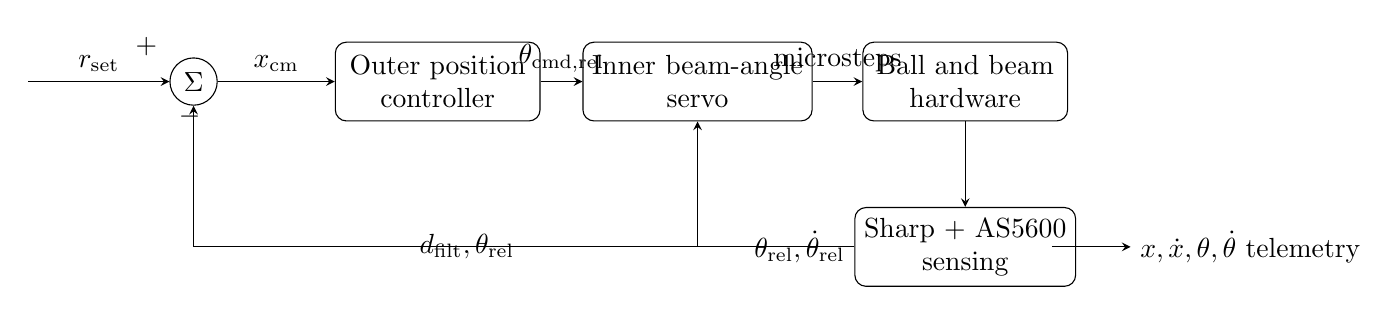
\begin{tikzpicture}[
    block/.style={draw, rounded corners, minimum width=2.6cm, minimum height=1cm, align=center},
    sum/.style={draw, circle, inner sep=0pt, minimum size=6mm},
    > = stealth
  ]
    \node[sum] (sum1) at (0,0) {$\Sigma$};
    \node[block] (outer) at (3.1,0) {Outer position\\controller};
    \node[block] (inner) at (6.4,0) {Inner beam-angle\\servo};
    \node[block] (plant) at (9.8,0) {Ball and beam\\hardware};
    \node[block] (sensorx) at (9.8,-2.1) {Sharp + AS5600\\sensing};

    \draw[->] (-2.1,0) -- node[above] {$r_{\text{set}}$} (sum1);
    \draw[->] (sum1) -- node[above] {$x_{\text{cm}}$} (outer);
    \draw[->] (outer) -- node[above] {$\theta_{\text{cmd,rel}}$} (inner);
    \draw[->] (inner) -- node[above] {microsteps} (plant);
    \draw[->] (plant) -- (sensorx);
    \draw[->] (sensorx.west) -| node[pos=0.25,left] {$d_{\text{filt}},\theta_{\text{rel}}$} (sum1.south);
    \draw[->] (sensorx.west) -| node[pos=0.35,right] {$\theta_{\text{rel}},\dot{\theta}_{\text{rel}}$} (inner.south);
    \draw[->] (10.9,-2.1) -- ++(1.0,0) node[right] {$x,\dot{x},\theta,\dot{\theta}$ telemetry};
    \node at (-0.6,0.45) {$+$};
    \node at (-0.05,-0.45) {$-$};
  \end{tikzpicture}
  \caption{Implementation-oriented cascaded control structure used by the April 11
  telemetry run.}
  \label{fig:cascade_block}
\end{figure}

\subsection{Inner Beam-Angle Servo}

The commanded beam angle is first limited to the calibrated soft window
$[-0.90,\ 3.30]$ degrees around the balance reference. The beam-angle error is

\begin{equation}
  e_{\theta,\text{deg}} = \theta_{\text{cmd,cal,deg}} - \theta_{\text{cal,deg}}
\end{equation}

If both the angle error and beam-rate magnitude are inside the deadband,
$|e_{\theta}| \le \SI{0.040}{deg}$ and
$|\dot{\theta}_{\text{deg/s}}| \le \SI{0.60}{deg/s}$, the controller outputs zero
steps. Otherwise the discrete servo computes

\begin{equation}
  \text{raw\_steps}[k] =
  -\left(0.70\,e_{\theta,\text{deg}}[k]\right)\cdot 115.9399
  + \text{residual}[k-1]
\end{equation}

and rounds the result to an integer command clipped to $\pm 40$ microsteps per cycle.

\subsection{Outer Ball-Position Law}

The outer loop clamps the derivative states to

\begin{equation}
  |x_{\dot{\text{cm/s}}}| \le \SI{4.50}{cm/s},
  \qquad
  |\theta_{\dot{\text{deg/s}}}| \le \SI{4.0}{deg/s}
\end{equation}

and then applies the tuned state-feedback law

\begin{equation}
  \theta_{\text{fs,cmd,deg}}
  = g_{\text{outer\_sign}}
    \left(
      k_x x_{\text{cm}}
      + k_v x_{\dot{\text{cm/s}}}
      + k_t \theta_{\text{rel,deg}}
      + k_{\omega} \theta_{\dot{\text{deg/s}}}
      + i_{\text{term,deg}}
    \right)
\end{equation}

with the April 11 defaults

\begin{align}
  g_{\text{outer\_sign}} &= -1 \\
  k_x &= 0.28 \\
  k_v &= 0.20 \\
  k_t &= 0.00 \\
  k_{\omega} &= 0.00 \\
  k_i &= 0.020
\end{align}

The integral state is constrained to the near-target capture region and clipped so that
$|i_{\text{term,deg}}| \le \SI{0.18}{deg}$.

\subsection{Recovery and Trim Logic}

The implementation retains three important practical features:

\begin{itemize}
  \item a \textbf{recovery floor} that enforces a minimum corrective beam command when
  the ball appears stalled away from the setpoint,
  \item a \textbf{zero-trim estimator} that logs a slow local balance-angle estimate
  under tight near-equilibrium conditions, and
  \item a \textbf{position-trim map} that can learn a local hold-angle bias across the
  usable setpoint range.
\end{itemize}

No learned position-trim feedforward was active during the April 11 run, so the
telemetry shows \verb|theta_trim_ff_deg = 0| for every row.

\section{Implementation Constants}

Table~\ref{tab:implementation_constants} compresses the runtime constants most relevant
to reproducing the telemetry run.

\small
\begin{longtable}{@{}p{0.19\linewidth}p{0.27\linewidth}p{0.14\linewidth}p{0.30\linewidth}@{}}
\caption{Key runtime constants from the firmware implementation in \texttt{src/main.cpp}.}
\label{tab:implementation_constants}\\
\toprule
Group & Constants & Value & Meaning \\
\midrule
\endfirsthead
\toprule
Group & Constants & Value & Meaning \\
\midrule
\endhead
\bottomrule
\endfoot
Timing & \verb|LOOP_MS|, \verb|DT| & \SI{40}{ms}, \SI{0.040}{s} & Main control cadence \\
Distance window & \verb|D_MIN_CM|, \verb|D_MAX_CM|, \verb|D_SETPOINT_DEFAULT_CM| & \SI{4.40}{cm}, \SI{12.66}{cm}, \SI{8.53}{cm} & Allowed sensing and default center setpoint \\
Sharp fit & \verb|SHARP_FIT_K_V_CM|, \verb|SHARP_FIT_OFFSET_CM| & 12.25, -0.62 & Inverse-voltage distance calibration \\
Angle calibration & \verb|THETA_SLOPE_DEG_PER_AS_DEG|, \verb|THETA_OFFSET_DEG| & 0.07666806, -23.28443907 & Online AS5600 to beam-angle affine fit \\
Angle limits & \verb|THETA_CAL_MIN_DEG|, \verb|THETA_CAL_MAX_DEG| & -0.70, 3.10 & Measured calibrated beam-angle range \\
Stepper conversion & \verb|STEPS_PER_REV|, \verb|STEPS_PER_BEAM_DEG| & 3200, 115.9399 & Empirical beam-angle to microstep conversion \\
Inner loop & \verb|INNER_KP_THETA|, \verb|INNER_KD_THETA|, \verb|INNER_MAX_STEP_DELTA| & 0.70, 0.00, 40 & Discrete beam-angle servo gains and step clamp \\
Outer loop & \verb|OUTER_KX_DEFAULT|, \verb|OUTER_KV_DEFAULT|, \verb|OUTER_KI_DEFAULT| & 0.28, 0.20, 0.020 & Default position-feedback and integral gains \\
Recovery & \verb|RECOVERY_ENTER_X_CM|, \verb|RECOVERY_FLOOR_DEFAULT_DEG|, \verb|RECOVERY_FLOOR_MAX_DEG| & \SI{1.20}{cm}, \SI{0.70}{deg}, \SI{1.10}{deg} & Stall detection and minimum corrective angle floor \\
Staircase & \verb|STAIRCASE_STAGE_MS|, \verb|STAIRCASE_FAR_SETPOINT_CM|, \verb|STAIRCASE_CENTER_SETPOINT_CM|, \verb|STAIRCASE_NEAR_SETPOINT_CM| & \SI{20000}{ms}, 12.16, 8.53, 4.90 & Built-in experiment sequence used in the telemetry log \\
\end{longtable}
\normalsize

% !TEX root = ../main.tex
\chapter{Beam-Angle Calibration Analysis}

This chapter analyzes the combined forward and reverse calibration data stored in
\path{calibration_logs/combined_20260407_forward_reverse/combined_cleaned_calibration.csv}.
Those data are used here as the direct source for beam-angle calibration figures and
hysteresis statistics.

\section{Scope of the Calibration Data}

The combined CSV merges a forward sweep and an interpolated reverse sweep onto a common
AS5600 angle grid. Its role in this report is to show the measured static beam-angle
relationship and the amount of direction-dependent hysteresis. It is not the runtime
controller source-of-truth by itself.

The implemented controller still uses the same-session affine calibration documented in
\path{modeling.md} and \path{src/main.cpp}:

\begin{equation}
  \theta_{\text{cal,deg}} = 0.07666806 \cdot \theta_{\text{AS5600,deg}} - 23.28443907
\end{equation}

That distinction matters because the combined forward/reverse dataset shows larger
direction-dependent offset than the same-session calibration chosen for closed-loop
control.

\section{Calibration Summary}

The combined CSV contains \CalibrationPointCount{} grid points. The observed reverse
minus forward hysteresis is summarized by:

\begin{itemize}
  \item mean hysteresis: \CalibrationMeanHysteresisDeg{} degrees,
  \item RMS hysteresis: \CalibrationRmsHysteresisDeg{} degrees, and
  \item max hysteresis: \CalibrationMaxHysteresisDeg{} degrees.
\end{itemize}

\ReportTableFromFile
  {Summary statistics generated directly from the combined calibration CSV.}
  {tables/calibration_summary.tex}
  {tab:calibration_summary}

\section{Forward/Reverse Curve}

\ReportFigure[width=0.95\linewidth]
  {figures/calibration_curve.pdf}
  {Forward and reverse beam-angle calibration curves generated directly from the
  combined calibration CSV. The overlaid affine line is the runtime mapping used in the
  controller.}
  {fig:calibration_curve}

Figure~\ref{fig:calibration_curve} shows that the relationship is approximately affine
over the operating window but not perfectly single-valued when travel direction is
considered. The combined dataset therefore serves best as an offline characterization
tool.

\section{Hysteresis Plot}

\ReportFigure[width=0.95\linewidth]
  {figures/calibration_hysteresis.pdf}
  {Direction-dependent hysteresis, plotted as reverse minus forward beam angle versus
  unwrapped AS5600 angle.}
  {fig:calibration_hysteresis}

The hysteresis remains positive across the combined dataset, with a magnitude large
enough to justify separating the thesis-facing static characterization from the simpler
runtime affine map used for controller execution.

% !TEX root = ../main.tex
\chapter{Experiment Results}

\section{Telemetry Mapping and Analysis Assumptions}

The results in this chapter come from
\path{telemetry_logs/20260411_142117/telemetry.csv}. The analysis script uses the
logged columns \verb|t_ms|, \verb|setpoint_cm|, \verb|d_filt_cm|, \verb|x_cm|,
\verb|x_dot_cm_s|, \verb|theta_rel_deg|, \verb|theta_dot_deg_s|,
\verb|theta_cmd_rel_deg|, \verb|mode|, \verb|valid|, \verb|driver_enabled|,
\verb|recovery_active|, \verb|step_pos|, and \verb|step_delta|.

Only rows with \verb|mode == 2| and \verb|driver_enabled == 1| are treated as
closed-loop experiment data. Position-derived metrics also honor the logged
\verb|valid| flag because the far-step segment contains intermittent invalid Sharp
samples.

For figure readability, the position and error plots use a display-only five-sample
centered rolling mean of the logged position signal, and short interior invalid gaps
are bridged only in the drawn trace. The summary tables and reported metrics still use
the raw valid samples from the CSV.

\ReportTableFromFile
  {Signal mapping assumptions used by the analysis pipeline.}
  {tables/signal_mapping.tex}
  {tab:signal_mapping}

\section{Run Summary}

The full log contains \TelemetryRowCount{} rows spanning \TelemetryDurationSeconds{}
seconds, with \TelemetryClosedLoopRowCount{} rows in closed-loop cascade mode. The run
contains \TelemetryInvalidRowCount{} invalid sensor rows and \TelemetryRecoveryRowCount{}
rows with recovery active. The maximum observed absolute tracking error was
\TelemetryMaxAbsErrorCm{} cm, while the maximum measured beam-angle magnitude and
command magnitude were \TelemetryMaxBeamAngleDeg{} deg and \TelemetryMaxCommandDeg{}
deg respectively.

\ReportTableFromFile
  {Run-level summary generated from the telemetry CSV.}
  {tables/telemetry_run_summary.tex}
  {tab:telemetry_run_summary}

\section{Overview Plot}

\ReportFigure[width=\linewidth]
  {figures/telemetry_overview.pdf}
  {Phase-by-phase overview of the staircase experiment. Each panel uses a local time
  axis and its own vertical scale so the hold portions remain readable. The bold red
  curve is a display-smoothed version of the valid measured signal, while the faint raw
  trace shows the underlying sensor fluctuation.}
  {fig:telemetry_overview}

The staircase sequence consists of an initial center hold, a far-side step, a return to
center, and a near-side step. The local time axes make the settled portions legible
without altering the underlying data. Validity losses are concentrated in the far-side
segment, which is why the generated summary tables separate valid sample counts from
total row counts.

\section{Ball-Position Tracking}

\ReportFigure[width=\linewidth]
  {figures/telemetry_position_tracking.pdf}
  {Reference tracking by commanded transition. The left column shows the first
  \SI{8}{s} after each setpoint change, while the right column zooms into the late hold
  portion of the same segment.}
  {fig:telemetry_position_tracking}

\ReportFigure[width=\linewidth]
  {figures/telemetry_tracking_error.pdf}
  {Late-hold tracking error
  $x_{\text{cm}} = d_{\text{filt,cm}} - d_{\text{setpoint,cm}}$ for each commanded
  transition. Dashed lines show the default settling band used in the summary metrics,
  while the bold curve uses the same display-only smoothing as the position plots.}
  {fig:telemetry_tracking_error}

The split transition-and-hold layout makes the experiment easier to read than a single
long time axis. In particular, the far-side and near-side moves show usable late-hold
tracking once the initial transport transient is separated from the rest of the phase.
The center-return segment still carries the largest residual offset in the available
window, so the figure presentation is clearer but not artificially optimistic.

\section{Beam Motion and Control Effort}

\ReportFigure[width=\linewidth]
  {figures/telemetry_beam_angle.pdf}
  {Measured beam angle versus time during the staircase experiment.}
  {fig:telemetry_beam_angle}

\ReportFigure[width=\linewidth]
  {figures/telemetry_control_input.pdf}
  {Final relative beam-angle command sent to the inner loop.}
  {fig:telemetry_control_input}

\ReportFigure[width=\linewidth]
  {figures/telemetry_velocity_rate.pdf}
  {Ball velocity and beam-angle rate estimates derived from the logged telemetry.}
  {fig:telemetry_velocity_rate}

The logged beam-angle command remains well inside the configured \SI{2.0}{deg} command
cap, and the CSV shows \verb|theta_cmd_sat = 0| for all rows. Recovery activates only
briefly during large transitions, which is consistent with the firmware design intent:
use recovery as a minimum-corrective-angle floor rather than as the dominant transport
mechanism.

\section{Performance Metrics}

\ReportTableFromFile
  {Per-step tracking metrics computed from valid closed-loop samples. Settling uses the
  default band $\max(\SI{0.2}{cm}, 5\%$ of commanded step size$)$. Unsupported metrics
  remain \texttt{N/A}.}
  {tables/telemetry_step_metrics.tex}
  {tab:telemetry_step_metrics}

The step metrics confirm three main points:

\begin{itemize}
  \item the far-side transition is limited by invalid distance samples and does not
  reach a clean settled condition in the available segment length,
  \item the center-return and near-side transitions achieve finite rise times but still
  show non-negligible residual error over the final valid window, and
  \item the recorded experiment is more useful as a realistic tuning baseline than as a
  final high-performance demonstration.
\end{itemize}

% !TEX root = ../main.tex
\chapter{Conclusion}

This report system turns the repository into a self-contained ball and beam experiment
record. It packages the mathematical model, runtime controller description, calibration
analysis, telemetry plots, generated tables, and local build tooling into a single
maintainable LaTeX tree under \path{report/}.

From the experiment itself, the main conclusions are:

\begin{itemize}
  \item the nonlinear model and linearized operating-point analysis remain consistent
  with the staged cascaded controller architecture,
  \item the combined forward/reverse calibration data expose measurable hysteresis, so
  offline calibration analysis should remain distinct from the simpler online affine
  mapping used by the firmware, and
  \item the April 11 staircase run demonstrates functional closed-loop transport across
  the usable sensing window, but the response quality is still limited by sensor
  invalidity and residual steady-state error during larger moves.
\end{itemize}

Immediate next steps are to collect cleaner far-side telemetry, improve near/far
distance validity robustness, and rerun the staircase experiment after those sensing
improvements so the same report pipeline can produce a higher-confidence final results
chapter.


\ReportPrintBibliography

\end{document}
